\documentclass[a4paper]{article}
% generated by Docutils <http://docutils.sourceforge.net/>
\usepackage{fixltx2e} % LaTeX patches, \textsubscript
\usepackage{cmap} % fix search and cut-and-paste in Acrobat
\usepackage{ifthen}
\usepackage[T1]{fontenc}
\usepackage[utf8]{inputenc}
\usepackage{lmodern}

\usepackage{graphicx}
\usepackage{placeins}
\usepackage{subfigure}
\usepackage{xcolor}

\usepackage{hyperref}

\newcommand{\tag}[1]{
\sffamily
\fcolorbox[RGB]{200,192,144}{200,248,200}{\textbf{#1}}
\normalfont
}

\newcommand{\ie}{{\textit{i.e.\ }}}
\newcommand{\cf}{{\textit{cf\ }}}
\newcommand{\eg}{{\textit{e.g.\ }}}
\newcommand{\behaviour}{{\item \textbf{Possible behaviour:~}}}



%%% Title Data
\title{Towards a new intermediate layer for geometric and temporal representation}

\author{Séverin Lemaignan et al.}
\date{}


%%% Body
\begin{document}
\maketitle

{\color{red} Warning: this document is a working draft. Many sections are still incomplete.}

\section*{Report overview}

This report aims at clarifying the challenges we currently face regarding
geometric and time representation on the robots, and summarizing the
existing and proposed directions to address these challenges.

This report is organized as follow:

\begin{itemize}
    \item first, we present in broad terms the problem we try to solve,

    \item  then, we present a set of use-cases that underline the limitation of
        our current tools and hint to the new capabilities we want to endow our
        robots with,

    \item from these use-cases, we isolate a set of expected features for the
        software system we want to design,

    \item the fourth section present a (currently largely incomplete) review of
        existing art,

    \item we present in the next section a set of early designs and proposals
        from the last year of discussions on this subject

    \item finally, we present the {\tt libworlds} proposal, an attempt at synthesizing
        the previous ideas.

\end{itemize}

We conclude the report with a proposal for a development road-map.

\clearpage
%___________________________________________________________________________

\section{Problem Statement}
\label{problem-statement}%

In the stack of software components required for an autonomous robot, the
layer that provide an uniform representation of the robot's environment not
only suitable, but even convenient for decision making, is crucial.

Because both the sensors inaccuracies and the dynamic nature of the world
(objects and structures constantly appear and disappear), this layer needs to
accommodate unexpected changes and filter out as much noise introduced by faulty
perception as possible, which also require the maintenance of an history of
the successive world states.

Also, this layer must remain as light as possible for the software components
built on top of it.  These upper layers include components for geometric
reasoning, temporal reasoning/action recognition, geometric motion planner,
symbolic task planners (that need to control the geometric feasibility of a
plan), learning modules and maybe others.

Figure~\ref{fig|saphari} gives a real world example of a (proposed)
architecture for a modern, interactive robot, from the SAPHARI project. The
representation layer we are designing would enable the efficient implementation
of several of the cognitive capabilities that appear on the diagram.

\begin{figure}[!h]
    \centering
    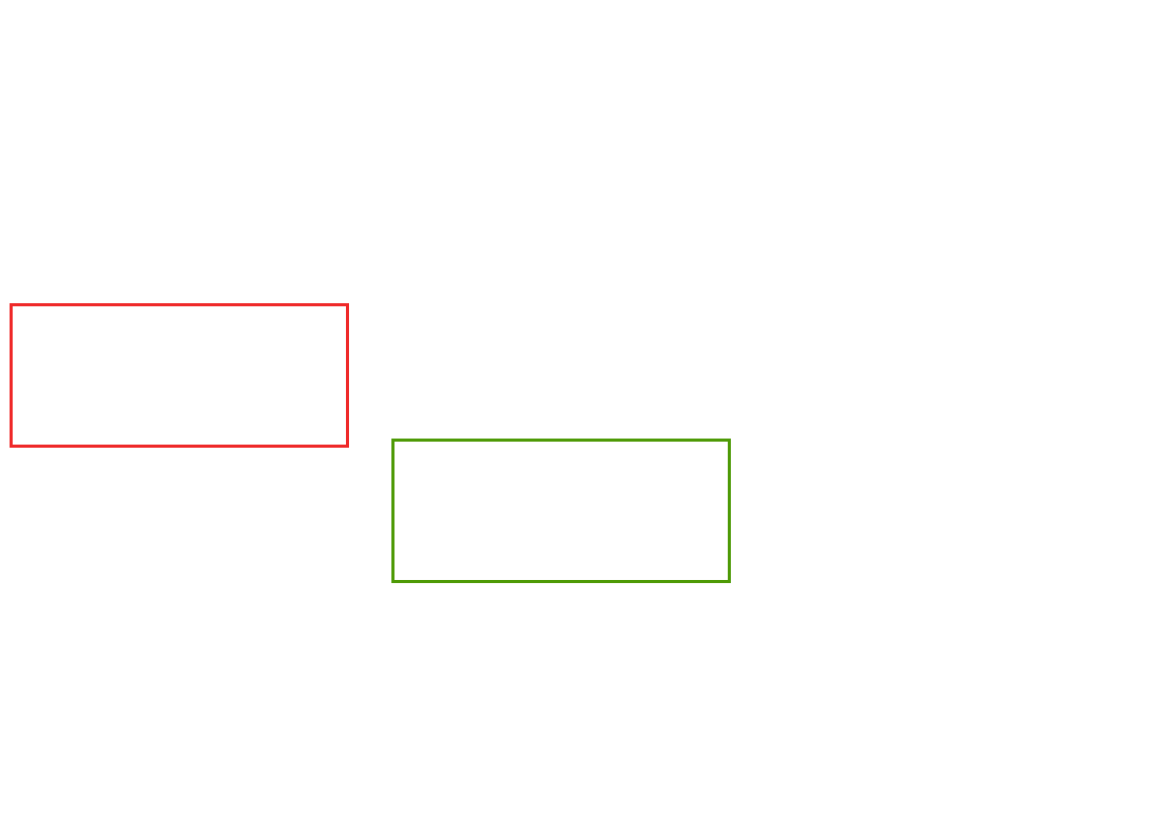
\includegraphics[width=\columnwidth]{images/saphari-focused.pdf}

    \caption{Draft of a proposed architecture for the European SAPHARI project.
    We aim at \emph{supporting} in a convenient and efficient way the implementation of the
    functions in the red block, based on inputs from the green block.}

    \label{fig|saphari}
\end{figure}


The geometric and temporal representation layer is only an intermediate tool
used by higher cognitive functions through an API: it must feel light,
convenient, efficient to use.  The less we think about it, the better.

This does not mean it does a simple job. Amongst the challenging tasks we have
identified, we can mention:

\begin{itemize}
    \item ensuring physically realistic model of the world (also known as the
        "flying video tapes" issue)

    \item managing several level of refinement of object's model (from partial
        point clouds to accurate CAD models)

    \item managing plausible states for unseen/not visible/occluded objects
        (probabilistic modeling, physics reasoning)

    \item managing world discontinuities (\eg, one single blob turns out to be
        two different objects, next to each other)

    \item representing suppositions (\eg a human tells the robot that a box is behind him)

    \item representing fields (\eg the field of reachability of an object for
        an agent, a traversability map, etc.)


\end{itemize}

Even if some of these tasks are not achieved in the first versions of the
project, we want to develop a software architecture that makes it possible to
implement at some point this kind of features.

\section{Use-cases}
\label{use-cases}%

For each case, labels indicates which aspects are involved: \tag{world
building}, \tag{geometric reasoning}, \tag{temporal reasoning}

Feel free to also submit new use-cases if you think they are not already covered.

%___________________________________________________________________________

\subsection{ an object is not perceived anymore, but stays in the model and ``floats in the air''%
  \label{case-1-an-object-is-not-perceived-anymore-but-stays-in-the-model-and-floats-in-the-air}%
}

\tag{world building}
%
\begin{quote}
%
\begin{itemize}

\behaviour We want the object position to be filtered based on physical constraints (like gravity, or possible trajectory - taking into account previous speed)

\end{itemize}

\end{quote}


%___________________________________________________________________________

\subsection{ an agent grasps an object. The object is not visible anymore%
  \label{case-2-an-agent-grasps-an-object-the-object-is-not-visible-anymore}%
}

\tag{world building}
\tag{geometric reasoning}
%
\begin{quote}
%
\begin{itemize}

\behaviour If we know the grasp was successful, then simply attach the object to the end effector

\behaviour If we see again the object, far from the end effector, assume the grasp failed

\end{itemize}

\end{quote}

(cf also case 5)


%___________________________________________________________________________

\subsection{The perception routines are slightly unstable, objects keep moving around a bit%
  \label{case-3-the-perception-routines-are-slightly-unstable-objects-keep-moving-around-a-bit}%
}

\tag{world building}
%
\begin{quote}
%
\begin{itemize}

\behaviour Implement proper dynamic filtering (low-pass filter)

\end{itemize}

\end{quote}


%___________________________________________________________________________

\subsection{The perception routines are strongly unstable, objects jump around%
  \label{case-4-the-perception-routines-are-strongly-unstable-objects-jump-around}%
}

\tag{world building}
%
\begin{quote}
%
\begin{itemize}

\behaviour Implement proper geometric filtering, possibly coupled with physical
simulation to check if a large displacement is actually physically possible

\end{itemize}

\end{quote}


%___________________________________________________________________________

\subsection{A object is perceived to be slightly INSIDE another one. Symbolic reasoning tells it is actually on top of it%
  \label{case-5-a-object-is-perceived-to-be-slightly-inside-another-one-symbolic-reasoning-tells-it-is-actually-on-top-of-it}%
}

\tag{world building}
\tag{geometric reasoning}
%
\begin{quote}
%
\begin{itemize}

\behaviour Geometric reasoning should be allowed to provide feedback to the
filtering routines to alter the model based on reasoning (cf also case 2)

\end{itemize}

\end{quote}


%___________________________________________________________________________

\subsection{The robot wants to predict ``what happen if I drop this object''%
  \label{case-6-the-robot-wants-to-predict-what-happen-if-i-drop-this-object}%
}

Equivalent use case: an object has disappeared, the robot wants to have ideas where to look for it.
\tag{geometric reasoning}
%
\begin{quote}
%
\begin{itemize}

\behaviour Endow to robot with a physics engine that can be queried to compute
possible positions for given objects in the future.

\end{itemize}

\end{quote}

%___________________________________________________________________________

\subsection{Compute symbolic relationships between objects, even when many objects are present.}


\tag{geometric reasoning}
%
\begin{quote}
%
\begin{itemize}

\behaviour Develop what is currently done in SPARK, allow computation symbolic relations like isIn,
IsOn, isNextTo, isInFrontOf. Ease the addition of new relations. Note that 'in front of', for instance,
requires that a 'front face' exist.

\behaviour Implement heuristics and/or strategies (like lazy evaluation) to
efficiently scale when the amount of objects increase.

\end{itemize}

\end{quote}


%___________________________________________________________________________

\subsection{What is visible/reachable for each agents?%
  \label{case-7-what-is-visible-reachable-for-each-agents}%
}

\tag{geometric reasoning}
%
\begin{quote}
%
\begin{itemize}

\behaviour Allow perspective taking (move the point of view from one agent to another one).

\behaviour Expose an efficient API for inverse kinematics and collision
checking that should allow reachability testing.

\end{itemize}

\end{quote}


%___________________________________________________________________________

\subsection{The human says: ``there's a black box behind you''. The robot add it somehow%
  \label{case-8-the-human-says-there-s-a-black-box-behind-you-the-robot-add-it-somehow}%
}

\tag{geometric reasoning}
\tag{world building}

This ability is sometimes referred as \emph{Presupposition Accommodation}:
ability to assume a fact to be true, even without explicit prior sensing. Cf
\url{http://en.wikipedia.org/wiki/Presupposition\#Accommodation_of_presuppositions}
and \cite{Mavridis2005}
%
\begin{quote}
%
\begin{itemize}

\behaviour add support for presupposition accomodation (which implies the
ability for the geometric reasoning to alter the world model)

\end{itemize}

\end{quote}


%___________________________________________________________________________

\subsection{The robot wants to go from A to B, but clutter on the ground prevent it. We want the robot to first remove hindering objects%
  \label{case-9-the-robot-wants-to-go-from-a-to-b-but-clutter-on-the-ground-prevent-it-we-want-the-robot-to-first-remove-hindering-objects}%
}

This use case requires external symbolic and geometric planing that is out of
the scope of the project. But the project should provide representations useful to solve
this kind of issue.

\subsection{Monitor back channel communication on a human}

This includes nodding, quick glances, etc.

\tag{geometric reasoning}
\tag{temporal reasoning}

\begin{quote}
%
\begin{itemize}

\behaviour we want to be able to describe some subtle behaviours as a set of temporal and geometric fine-grained constraints. When they are recognized, these behaviours should be notified back to a controller.

\end{itemize}

\end{quote}



%%%%%%%%%%%%%%%%%%%%%%%%%%%%%%%%%%%%%%%%%%%%%%%%%%%%%%%%%%%%%%%%%%%%%%%%%%%%%%
%%%%%%%%%%%%%%%%%%%%%%%%%%%%%%%%%%%%%%%%%%%%%%%%%%%%%%%%%%%%%%%%%%%%%%%%%%%%%%
%%%%%%%%%%%%%%%%%%%%%%%%%%%%%%%%%%%%%%%%%%%%%%%%%%%%%%%%%%%%%%%%%%%%%%%%%%%%%%

\section{Expected features}

This section is still incomplete.

\subsection{Temporal reasoning}

\begin{itemize}
    \item Many properties need to be assessed on a short time frame.
        The project must offer an easy way to access to delayed and/or
        filtered geometric properties of the scene.

    \item Idea of sliding time windows to monitor certain states, that
        could be dynamically modified (length, granularity...) 

\end{itemize}

\subsection{Alteration of the 3D model based on geometric reasoning}


The outcomes of the reasoning should be possibly used to alter the 3D
model. For instance: a box is computed to be on another one, but perception
returns boxes are partially overlapping. The project should be able to update a
consolidated 3D model of the environment. 

\subsection{Technical aspects}

\subsubsection{Performances}

The libraries are likely to require a fair amount of computing resources (for
computations like IK, collision checking..., and for storage of models).

The design of the system must ensure that:
\begin{itemize}
    \item it makes use of multi-core architectures

    \item it remains open to the use of GPGPU approaches where relevant tasks
        (\ie, heavy computations must be isolated in replaceable modules)

\end{itemize}

Furthermore, because the system will share its world model with several client
simultaneously, a special care must be put on the design of the communication
layer.


\subsubsection{Good modularity/extensibility}

Good software practises encourage modular design, in particular because it
eases software maintenance.

Because 1) our research environment leads to a strong student turn-over, 2) the
development of the project is likely to be incremental, with evolving technical
choices, it is absolutely crucial to adopt a carefully designed modular
architecture.

Amongst other things, this design should:

\begin{itemize}
    \item not commit to a single technology

    \item fast prototyping (via a plugin and/or scripting interface)

    \item an (reasonably) easy switch of key libraries (communication, physics
        engine, serialization, meshes import, collisions...)

\end{itemize}

\section{Prior art}

This section is still incomplete.

\subsection{SPARK}

In this section we present SPARK (\emph{SPAtial
Reasoning \& Knowledge}~\cite{Sisbot2011}), a situation assessment reasoner
that generates symbolic knowledge from the geometry of the environment with
respect to relations between objects, robots and humans, also taking into
account the different perspective that each agent has on the environment.

SPARK can be seen as an amodal geometric model of the environment that serves
both as basis for the fusion of the perception modalities and as bridge with
the symbolic layer.

Figure~\ref{fig|spark} shows a screenshot of the SPARK environment side-by-side
with the real environment. In this example, objects are
identified and localised through 2D barcodes. The human pose is tracked with
a Kinect-like device (assisted by motion capture to accurately track the
head motion, which is required to compute what the human is looking at).

The geometric model is continuously updated at run-time by the robot.

One of the main strenght of SPARK is its ability to perform \emph{perspective
taking}, \ie to analyse the environment from the point of view of each of the
agent present in the scene.

Spatial perspective taking refers to the qualitative spatial location of
objects (or agents) with respect to a frame (\eg \emph{the keys on my left}).
Based on this frame of reference, the description of an object
varies~\cite{Marin2008}. Humans mix perspectives frequently during interaction.
This is more effective than maintaining a consistent one, either because the
(cognitive) cost of switching is lower than remaining with the same
perspective, or if the cost is about the same, because the spatial situation
may be more easily described from one perspective rather than
another~\cite{Tversky1999}. Ambiguities arise when one speaker refers to an
object within a reference system (or changes the reference system, \ie switches
perspective) without informing his/her partner about it~\cite{Breazeal2006,
Ros2010}. For example, the speaker could ask for the ``keys on the left''.
Since no reference system has been given, the listener would not know where
exactly to look.  However, asking for ``the keys on your left'' gives enough
information to the listener to understand where the speaker is referring to. On
the contrary, when using an exact, unambiguous term of reference to describe a
location (\eg. ``go north'') no ambiguity arises.

In this work, we use two types of the frames of reference: egocentric (from the
robot perspective) and addressee-centred (from the human perspective).

\begin{figure}[ht!]
   \begin{center}
%
       \subfigure{
           \includegraphics[width=0.5\textwidth]{images/etat.jpg}
       }%
       \subfigure{%
          \includegraphics[width=0.43\textwidth]{images/etat_spark.png}
       }\\ %  ------- End of the first row ----------------------%
%
   \end{center}

   \caption{The robot represents at run-time its environment in a 3D model
   resulting of the sensors' inputs fusion (Kinect, motion capture, 2D barcodes
   tracking).}

   \label{fig|spark}

\end{figure}

\paragraph{Symbolic locations}

Human commonly refer to the positions of objects with symbolic descriptors
(like \emph{on}, \emph{next to}...) instead of precise, absolute positions.
These type of descriptors have been studied in the context of language
grounding \cite{O'Keefe1999,Matuszek2010,Regier2001,Kelleher2006,Blisard2005}.
In SPARK we focus agent-independent symbolic locations and agent-dependent,
relative locations.

\paragraph{Agent-independent locations}

We can refer to object locations with respect to other objects in the
environment, such as \emph{above, next to, in}, etc. SPARK computes
three main relations based on the bounding box and centre of mass of the
objects (fig.~\ref{fig|sprelations}): 

\begin{itemize}
	\item \texttt{isOn}: computes if an object $O_1$ is on another object $O_2$ by
	evaluating the center of mass of $O_1$ according to the bounding box of $O_2$.

	\item \texttt{isIn}: evaluates if an object $O_1$ is inside another object
	$O_2$ based on their bounding boxes $BB_{O_1}$ and $BB_{O_2}$.

	\item \texttt{isNextTo}: indicates whether an object $O_1$ is next to another
	object $O_2$. We cannot use a simple distance threshold to determine if two
	objects are next to each other since the relation is highly dependent on the
	dimensions of the objects. For instance, the maximum distance between large
	objects (\eg two houses) to consider them as being next to each other is much
	larger than the maximum distance we would consider for two small objects (\eg
	two bottles). Thus, the relation between the dimensions and the distances of
	the objects are taken into account.  

\begin{figure} 
	\centering
	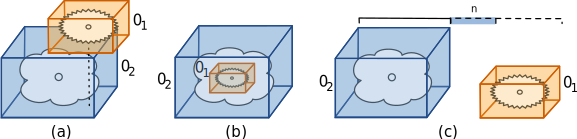
\includegraphics[width=0.95\columnwidth]{images/spatial_relation.pdf}
	\caption{Spatial relations between two objects: (a) \texttt{isOn} relation, 
	(b) \texttt{isIn} relation, and (c) \texttt{isNextTo} relation.} 
	\label{fig|sprelations} 
\end{figure}

\end{itemize} 

To ensure the different agent models are up-to-date, all these properties are
always computed on-line, each time the current state of the world changes.

SPARK also compute symbolic facts related to agent independent world dynamics.
The predicate \texttt{isMoving} states, for each tracked entity, whether it is
currently moving or not.


\paragraph{Agent-dependent placements}

While in previous section we listed several \emph{absolute} location predicate,
many topological relations are directly dependent from the observation point.

The predicate \texttt{hasRelativePosition} represents spatial locations
between agents and objects that are agent dependent.  We compute these spatial
locations by dividing the space around the referent (an agent) into $n$ regions
based on arbitrary angle values relative to the referent orientation.  For
example, for $n = 4$ we would have the space divided into \emph{front, left,
right} and \emph{back}. Additionally, two proximity values, \emph{near} and
\emph{far}, are also considered. The number of regions and proximity values can
be chosen depending on the context where the interaction takes place.

Through perspective taking, SPARK computes for each agent a symbolic
description of the relative positioning of objects in the environment.

\paragraph{Building a model of agents}
\label{sect|grounding_agents}

SPARK computes the following capabilities from the perspectives of each agent:

\begin{itemize}

\item \emph{Sees}: An important ability to know about an agent is to predict
\emph{What can it see?}, \ie what is within its field of view (FOV). Being able
to compute this information, the robot can reuse it for instance to infers
which object a human is searching for (the one that is not currently visible,
otherwise the user would not be searching for it).  In
figure~\ref{fig::sparkRepresentations}\emph{a} the field of view of a person is
illustrated with a grey cone (broader one). While he is able to see the two
small boxes on the table in front of him, the big box on his right is out of
his FOV, and therefore, he is not able to see it. 

\item \emph{Looks At}: this relation corresponds to what the agent is focused
on, \ie where its focus of attention is directed. This model is based on a
narrower field of view, the field of attention (FOA). 
Figure~\ref{fig::sparkRepresentations}\emph{a}
shows the field of attention of a person with a green cone (narrower one). In
this example only the grey box satisfies the \texttt{looksAt} relation.

\item \emph{Points At}: verifies whether an object is pointed at by an agent.
This relation is particularly useful during interaction when one of the agents
is referring to an object saying ``this" or ``that" while pointing at it.
 
If a larger object occludes a smaller one while an agent is pointing at them, the
outcome of the evaluation will result only in one relation, \ie \texttt{agent\_01
pointsAt object\_01} since the small one is not visible to the agent.  On the
contrary, if the small object is in front of the big one, then both objects
will satisfy the relation, which may generate an ambiguity (which object the
agent refers to?) that is let to be solved by other discrimination algorithms.

To make recognition more robust, these three first capabilities are filtered
with an hysteresis function at the geometric level.

\item \emph{Reachable}: it allows the robot to estimate the agent's capability
to reach an object, which is fundamental for task planning. For example, if the
user asks the robot to give him/her an object, the robot must compute a transfer
point where the user is able to get the object afterwards. 
Figure~\ref{fig::sparkRepresentations}\emph{b} shows different reachability postures for each object
on the table. In the example, the bottle and the box are both reachable for the
human, but the teddy bear is too far. Instead, from the robot's perspective,
the teddy bear is reachable, while the bottle is not.

\end{itemize}

\begin{figure*}[!t]
    \begin{center}
    \subfigure[]{
        \includegraphics[width=0.4\linewidth]{images/looks.jpg} 
    }
    \subfigure[]{
        \includegraphics[width=0.35\linewidth]{images/reach.jpg}
    }
    \caption{(a) Field of view (FOV) and the field of attention (FOA) of the
    human. (b) Different reaching postures for the human.}
    \label{fig::sparkRepresentations}
    \end{center}
\end{figure*} 


While the first three relations (\texttt{sees}, \texttt{looksAt} and
\texttt{pointsAt}) are computed through a model based approach, the latter one
is based on the Generalized Inverse Kinematics with pseudo inverse
method~\cite{Nakamura90,Baerlocher04} to find a posture for the
agent where its end-effector is at the centre of the object within a given
tolerance.

SPARK also compute the global posture of agents (lying, standing, sitting)
based on simple heuristics (the height of the head).


\subsection{GSM}
\label{sect|gsm}

GSM (for \emph{Grounded Situation Model})~\cite{Mavridis2006} is a knowledge
representation system primarily built to ``facilitate cross-modal
interoperability'',  especially in the context of verbal interaction with a
robot.

GSM does not rely on any formal language but rather on a layered data structure
(figure~\ref{fig|gsm}) that organises the surrounding world into agents and
relations between agents.  Each agent (any animate or inanimate object) is
attached to a physical model (made of \emph{body parts} that have properties
like their position, color, etc.) and a mental model (which is a recursively
embedded GSM, thus allowing a sort of theory of mind).

\begin{figure}[!h]
    \centering
    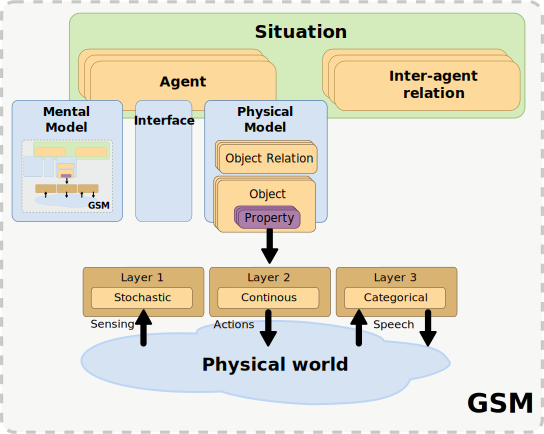
\includegraphics[width=0.65\columnwidth]{images/gsm.pdf}

    \caption{Simplified hierarchical structure of the Grounded Situation Model,
    based on~\cite{Mavridis2006}.}

    \label{fig|gsm}
\end{figure}

Properties are represented in three layers: a stochastic representation, close
to sensory percepts, a \emph{continuous single-valued} encoding of the
stochastic model, and a discrete, categorical model.

One notable feature of GSM is the \emph{bidirectionality} of the grounding
process: not only sensor percepts are abstracted into categories suitable for
human conversation, but human utterance (like ``There is a red ball in the
center of the table'') can also be turned into property descriptions. This
basically enable the knowledge representation system of the robot to
\emph{imagine} entities.

GSM also features several strategies for managing time and events.
\emph{Moments} are created by storing timestamped snap-shots of GSM, and
\emph{event classifiers} allow to define and detect events.

\paragraph{Experiments} GSM has mostly been tested on table-top manipulation
and interaction tasks (a ``conversational helping hand'' as stated by the
authors) implemented on a 7-DOF arm equipped with force feedback, cameras for blob
tracking and speech recognition (Sphinx4). Mavridis and Roy provide in addition
an in-depth analysis of the performance of GSM by the mean of a standard
psycholinguistic test, the \emph{Token test}~\cite{DiSimoni1978}.


\subsection{DyKnow}


%___________________________________________________________________________


\section{Previous proposals}

In this section, we present the various ideas/proposals that have been designed
and discussed over the last year. Some of them are very early designs, and are
only useful to understand how the project evolved and refined itself over time.

\subsection{Continuous merging}

\begin{figure}[!h]
    \centering
    \includegraphics[height=10cm]{images/spark_archi0.png}
    \caption{"Continous Merging" proposal}
    \label{fig|continousmerging}
\end{figure}

One of the issues we often encounter when building a geometric model of the
robot environment is caused by perception inaccuracies: some objects are
floating around, in irrealistic ways (typically because they are suddently not
percieved anymore).

This early proposal (figure \ref{fig|continousmerging}) introduce the idea of \textbf{physics-based reasoning} to
filter the geometric state: at each step, the future state (on ~100ms) of the
model is simulated by a physics engine, and we keep only the stable positions
of each entity.

\FloatBarrier

\subsection{Cascading filters}

\begin{figure}[!h]
    \centering
    \includegraphics[height=10cm]{images/spark_archi1.png}
    \caption{"Continous Merging" proposal}
    \label{fig|cascading}
\end{figure}


In this architecture (figure~\ref{fig|cascading}), a first module acquires and merge raw perception input,
and exposes the result as a "raw world state" poster/topic.

Then, a set of filters can be launched. They take one or several world model as
input and output a new, filtered, model. Amongst possible filters: a low-pass
one, another based on physics, etc.

Filters can be chained in any order, and can occur several times (for instance:
two low-pass filters, at different stage)

Finally, a special "geometric reasoning" module, that also act as a filter, is
in charge of computing symbolic facts from the geometric model.

It may embed its own physics engine for temporal projection ("what will happen
in the next 2 seconds if I drop the glass?") 

\FloatBarrier
\subsection{"Timeline centric" Architecture proposal}

\subsubsection{Cascading filters}

The main idea is, similarly to the proposal ''Cascading filters'', to have a
set of cascading filtering modules that expose successive world models.

A first module merges into a 3D models several 3D positions sources (ROS TF
trees in the diagram below, but this can be discussed) and there corresponding
meshes (from URDF or Collada).

\begin{figure}[!h]
    \centering
    \includegraphics[scale=0.5]{images/spark2_archi2_1.png}
\end{figure}

This is very similar to what RVIZ does for instance.

However, it could be extended with temporal filters (like Kalman filter) to
merge several sources for the same info (like 2 Kinects tracking the same
human).

This first raw 3D world model is exposed and reused by several
stabilization/filtering modules:

\begin{figure}[!h]
    \centering
    \includegraphics[scale=0.5]{images/spark2_archi2_2.png}
\end{figure}

Each filter outputs a new world model. Other module can thus work with a world
model at any level of filtering.

In the diagram above, I've put some example of possible filters:

\begin{itemize}
    \item the \textbf{low-pass} filter aim at removing simple perception noise (shakiness)
    \item the \textbf{physics-based} filter uses a physics engine to:
        \begin{itemize}
            \item filter out impossible movements,
            \item ensure physical consistency (no floating objects, no object inside another one)
            \item account for movement of non-visible objects that can be physically deducted (like A is in B, B moves => A moves with B) 
        \end{itemize}

    \item the \textbf{symbolic reasoning} filter implement filtering at an even higher level, for instance:
        \begin{itemize}
            \item If A is perceived at 2 distinct places, then... there's an issue!
            \item See also Nico Blodow paper, page 4-5 for example of symbolic reasoning on a geometric model. 
        \end{itemize}
\end{itemize}

With this architecture, new filters can be later easily added.

\FloatBarrier
\subsubsection{Timeline management}

This second proposal introduces the idea of a \emph{central timeline}. Every \emph{world
provider} (like filters) send to the timeline the changes:

\begin{figure}[!h]
    \centering
    \includegraphics[scale=0.5]{images/spark2_archi2_3.png}
\end{figure}

\FloatBarrier
The timeline can be in turn used by other modules (like an \textbf{action
recognition} module) to know when a certain event occurred. The timeline
clients describe the kind of temporal event they are interested in (like "the
PR2 head moved twice in the last 3 mins), and get triggered when such an event
occurs:

\begin{figure}[!h]
    \centering
    \includegraphics[scale=0.5]{images/spark2_archi2_4.png}
\end{figure}

Cf below for details on the timeline events system.

\FloatBarrier
\subsubsection{Reasoning on the world model}

The most stable world model can be used for various geometric reasoning tasks,
like perspective taking, geometric planing, simulation-based temporal
projection (cf paper by Lars Kunze, \cite{Kunze2011a}), etc.

\begin{figure}[!h]
    \centering
    \includegraphics[scale=0.5]{images/spark2_archi2_5.png}
\end{figure}

%___________________________________________________________________________

\FloatBarrier
\section{
  The Worlds proposal%
  \label{the-worlds-proposal}%
}


%___________________________________________________________________________

\subsection{
  Overview%
  \label{overview}%
}

This document presents a software framework (temporarly) called libworlds that
aims to update the current tools for geometric reasoning in use at
LAAS, and support current and future researches in this field.

The softwares that we introduce here are \emph{low-level} with respect
to the \emph{reasoning} tasks: they do not implement any high-level
geometric and/or temporal reasoning algorithms. Instead, they
focus on offering efficient low-level libraries to \emph{store} and
\emph{query} geometric and temporal models of the world (known to the
robot).

The framework is build around the idea of \emph{worlds}: each world
contains a geometric \emph{state} built by the robot (from its
perceptions or from computation applied on other models) and a
\emph{timeline} associated to this model that allow to access the model
back and forth in time:

\begin{itemize}

 \item the universe is describe as a set of \emph{worlds}, each of them comprise of a \emph{state} and 
 a \emph{timeline}. These worlds represent different perspectives 
 on the real world. They are meant to be easily created, exchanged, queried, compared.
   
 \item a \emph{state} is a model of the geometric and kinematic structure of the (current) world.
 It stores a set of kinematic chains and a set of meshes and physical properties associated to the joints
 of the kinematic chains. It can also represent fields of data (as a 2D map, discrete fields or continuous fields).
 It exposes services like collision checking.

 \item a \emph{timeline} that stores snapshots of the world's state at given timepoints. Thoses timepoints
 are defined by a set of \emph{event descriptors}. These descriptor use a particular grammar that implicitely 
 models which time-related concepts can be described.

 The timeline allows for jumping back in time (for temporal reasoning), or on the contrary move forward in time 
 (for planning purposes for instance).

\end{itemize}

%___________________________________________________________________________

\subsection{
  Terminology%
  \label{terminology}%
}

We call \emph{state} a set of kinematic chains (made from 0 to n
joints) that describe a geometric and kinematic organisation of
rigid bodies. The structure of the states is described below.

We call \emph{Current Geometric State} (CGS) the latest state which
is directly built from the sensors. It represents the physical
world, as perceived by the robot.

We call \emph{event} the specific state where the set of conditions
described by the \emph{event pattern} attached to the event is computed
to become true.
The grammar of the event patterns is described below.

We call \emph{timeline} a linear datastructure that stores pairs of
(timestamp, state) each time one of the events registered with the
timeline is triggered.

We call a \emph{world} a tuple (state, timeline, repository of event
patterns)

We call \emph{Current World} the world that contains the \emph{Current Geometric State}.


%___________________________________________________________________________

\subsection{
  libworlds API%
  \label{libworlds-api}%
}

libworlds exposes four APIs:
%
\begin{itemize}

\item the \emph{worlds API} allows to create a new or access an existing
world. When creating a new one, it can possibly be initialised
from another, existing one, and becomes then completely
independent: if altered (for planing, prediction, filtering...),
it does not impact the original world.

The API also allow to compare, diff and merge worlds with each others.

\item the \emph{states API} allows to alter and access a geometric state in
an efficient, thread- and process-safe way. This API is the main
entry point for sensor inputs and filters.

\item the \emph{event API} allows to register new events pattern: these
patterns are checked against the world's state, and when they
trigger, the current state is stored in the timeline (actually,
only a diff is stored). Events can be hierarchical, and the
patterns can refer to other, already defined, events.

\item the \emph{timeline API} lets users retrieve the state of the world at
certain time points in the past (either absolute or relative to
past events), or possibly in the future if future states are
available (after planning, for instance).

\end{itemize}


%___________________________________________________________________________

\subsection*{\phantomsection%
  Implementation%
  \addcontentsline{toc}{subsection}{Implementation}%
  \label{implementation}%
}


%___________________________________________________________________________

\subsubsection*{\phantomsection%
  Structure of states%
  \addcontentsline{toc}{subsubsection}{Structure of states}%
  \label{structure-of-states}%
}

A geometric state is stored as directed forests (a set of
directed graphs). Edges represent kinematic joints, while nodes
represent rigid bodies (soft bodies can not be represented in the
current state of this API).

Rigid bodies are represented as a structure containing:

%
\begin{itemize}

\item an unique identifier

\item their bouding boxes

\item a reference frame

\item a transformation matrix relative to the reference frame

\item the type of object (based on the robot ontology, default to ``Object'')

\item (optionally) a covariance matrix representing the uncertainty on the position and orientation of the body

\item (optionally) an (open) set of references to data representing the body (as described at the next section)

\end{itemize}

TBD: idea of fields (eg for Mightability Maps)?
TODO: efficient wrappers for OpenGL and collision detection


%___________________________________________________________________________

\subsubsection*{\phantomsection%
  Bodies library%
  \addcontentsline{toc}{subsubsection}{Bodies library}%
  \label{bodies-library}%
}

In order to minimise the size of the worlds' states, all data used
to represent a body (parametric model, meshes, point-clouds) are
stored in an external database (SQL, NoSQL? TBD), shared by all
worlds.

Each record in this database contains:
%
\begin{itemize}

\item an unique identifier (egal to the SHA1 of the dataset)

\item a code specifying the type and format of the dataset (TBD)

\item the actual dataset

\end{itemize}


%___________________________________________________________________________

\subsubsection*{\phantomsection%
  Timeline and state diffs%
  \addcontentsline{toc}{subsubsection}{Timeline and state diffs}%
  \label{timeline-and-state-diffs}%
}

TBD


%___________________________________________________________________________

\subsubsection*{\phantomsection%
  Events patterns%
  \addcontentsline{toc}{subsubsection}{Events patterns}%
  \label{events-patterns}%
}

Cf Vincent


%___________________________________________________________________________

\section{Development road-map}
\label{development-road-map}

\begin{enumerate}
    \item Implementation of the state API for a single world (the \emph{Current World}), including the \emph{bodies library} repository.
    \item Development of a first client to load 3D meshes and kinematic chains (based on the ASSIMP library)
    \item Development of a second client to display the state, based on TF and the existing visualisation capabilities of RVIZ.
    \item Support for NIUT and Viman
    \item Development of another client that exports the state as a SPARK poster
    \item Modification of SPARK to accept a world state from a poster
    \item Development of OpenGL and collision detection wrappers (Bullet?)
    \item Development of helpers to compute collisions
    \item Integration with ROS's table-top detector to acquire meshes
    \item Implementation of the events and timeline API
    \item Development of an efficient diffing algorithm
    \item Implementation of the Worlds API.
    \item Port of SPARK situation assessment to libworlds.
\end{enumerate}




%%%%%%%%%%%%%%%%%%%%%%%%%%%%%%%%%%%%%%%%%%%%%%%%%%%%%%%%%%%%%%%
\bibliographystyle{abbrv}
\bibliography{/home/slemaign/work/biblio/biblio_phd_severin}

\end{document}
